\newpage
\section{Fast Reduction}

\begin{align*}
p_{256} &= 2^{256} - 2^{224} + 2^{192} + 2^{96} - 1 \\
0 &\equiv 2^{256} - 2^{224} + 2^{192} + 2^{96} - 1 \pmod{p_{256}} \\
2^{256=32*8} &\equiv 2^{224} - 2^{192} - 2^{96} + 1 \pmod{p_{256}} \\
\\
2^{288=32*9} &\equiv 2^{256} - 2^{224} - 2^{128} + 2^{32} \pmod{p_{256}} \\
2^{288} &\equiv (2^{224} - 2^{192} - 2^{96} + 1) - 2^{224} - 2^{128} + 2^{32} \pmod{p_{256}} \\
2^{288} &\equiv - 2^{192} - 2^{128} - 2^{96} + 2^{32} + 1 \pmod{p_{256}} \\
\\
2^{320=32*10} &\equiv - 2^{224} - 2^{160} - 2^{128} + 2^{64} + 2^{32} \pmod{p_{256}} \\
\\
2^{352=32*11} &\equiv - 2^{256} - 2^{192} - 2^{160} + 2^{96} + 2^{64} \pmod{p_{256}} \\
2^{352} &\equiv - (2^{224} - 2^{192} - 2^{96} + 1) - 2^{192} - 2^{160} + 2^{96} + 2^{64} \pmod{p_{256}} \\
2^{352} &\equiv - 2^{224} - 2^{160} + 2\cdot 2^{96} + 2^{64} - 1 \pmod{p_{256}} \\
\\
2^{384=32*12} &\equiv - 2^{256} - 2^{192} + 2\cdot 2^{128} + 2^{96} - 2^{32} \pmod{p_{256}} \\
2^{384} &\equiv - (2^{224} - 2^{192} - 2^{96} + 1) - 2^{192} + 2\cdot 2^{128} + 2^{92} - 2^{32} \pmod{p_{256}} \\
2^{384} &\equiv - 2^{224} + 2\cdot 2^{128} + 2\cdot 2^{96} - 2^{32} - 1 \pmod{p_{256}} \\
\\
2^{416=32*13} &\equiv - 2^{256} + 2\cdot 2^{160} + 2\cdot 2^{128} - 2^{64} - 2^{32} \pmod{p_{256}} \\
2^{416} &\equiv - (2^{224} - 2^{192} - 2^{96} + 1) + 2\cdot 2^{160} + 2\cdot 2^{128} - 2^{64} - 2^{32} \pmod{p_{256}} \\
2^{416} &\equiv - 2^{224} + 2^{192} + 2\cdot 2^{160} + 2\cdot 2^{128} + 2^{96} - 2^{64} - 2^{32} - 1 \pmod{p_{256}} \\
\\
2^{448=32*14} &\equiv - 2^{256} + 2^{224} + 2\cdot 2^{192} + 2\cdot 2^{160} + 2^{128} - 2^{96} - 2^{64} - 2^{32} \pmod{p_{256}} \\
2^{448} &\equiv - (2^{224} - 2^{192} - 2^{96} + 1) + 2^{224} + 2\cdot 2^{192} + 2\cdot 2^{160} + 2^{128} - 2^{96} - 2^{64} - 2^{32} \pmod{p_{256}} \\
2^{448} &\equiv 3\cdot 2^{192} + 2\cdot 2^{160} + 2^{128} - 2^{64} - 2^{32} - 1 \pmod{p_{256}} \\
\\
2^{480=32*15} &\equiv 3\cdot 2^{224} + 2\cdot 2^{192} + 2^{160} - 2^{96} - 2^{64} - 2^{32} \pmod{p_{256}} \\
\end{align*}

\newpage
\noindent Consider $
Z=z_{15}\adjacent z_{14}\adjacent\cdots\adjacent z_0=\sum_{i=0}^{15}z_i2^{32i}\quad\text{with}\quad Z\in\intco{0, p_{256}^2}.
$

\begin{align*}
%z_0\cdot 2^{0=32*0} &= z_0\cdot (&&&&&&&&+1) \\
%z_1\cdot 2^{32=32*1} &= z_1\cdot (&&&&&&&+2^{32}&) \\
%z_2\cdot 2^{64=32*2} &= z_2\cdot (&&&&&&+2^{64}&&) \\
%z_3\cdot 2^{96=32*3} &= z_3\cdot (&&&&&+1\cdot 2^{96}&&&) \\
%z_4\cdot 2^{128=32*4} &= z_4\cdot (&&&&+1\cdot 2^{128}&&&&) \\
%z_5\cdot 2^{160=32*5} &= z_5\cdot (&&&+1\cdot 2^{160}&&&&&) \\
%z_6\cdot 2^{192=32*6} &= z_6\cdot (&&+1\cdot 2^{192}&&&&&&) \\
%z_7\cdot 2^{224=32*7} &= z_7\cdot (&+1\cdot 2^{224}&&&&&&&) \\
z_8\cdot 2^{256=32*8} &\equiv z_8\cdot (&+1\cdot 2^{224} &-1\cdot 2^{192}&&& -1\cdot 2^{96} &&&+ 1) \\
z_9\cdot 2^{288=32*9} &\equiv z_9\cdot (&&-1\cdot 2^{192}&& -1\cdot 2^{128} &-1\cdot 2^{96} &&+ 2^{32} &+ 1) \\
z_{10}\cdot 2^{320=32*10} &\equiv z_{10}\cdot (&- 1\cdot 2^{224}&& -1\cdot 2^{160} &-1\cdot 2^{128} &&+ 2^{64} &+ 2^{32}&) \\
z_{11}\cdot 2^{352=32*11} &\equiv z_{11}\cdot (&- 1\cdot 2^{224}&& -1\cdot 2^{160}&& + 2\cdot 2^{96} &+ 2^{64} &&- 1) \\
z_{12}\cdot 2^{384=32*12} &\equiv z_{12}\cdot (&- 1\cdot 2^{224}&&& + 2\cdot 2^{128} &+ 2\cdot 2^{96} &&- 2^{32} &- 1) \\
z_{13}\cdot 2^{416=32*13} &\equiv z_{13}\cdot (&- 1\cdot 2^{224} &+1\cdot 2^{192} &+ 2\cdot 2^{160} &+ 2\cdot 2^{128} &+1\cdot 2^{96} &- 2^{64} &- 2^{32} &- 1) \\
z_{14}\cdot 2^{448=32*14} &\equiv z_{14}\cdot (&&+3\cdot 2^{192} &+ 2\cdot 2^{160} &+1\cdot 2^{128} &&- 2^{64} &- 2^{32} &- 1) \\
z_{15}\cdot 2^{480=32*15} &\equiv z_{15}\cdot (&+3\cdot 2^{224} &+ 2\cdot 2^{192} &+1\cdot 2^{160} &&-1\cdot 2^{96} &- 2^{64} &- 2^{32}&)
\end{align*}
\begin{table}[h!]\centering
\begin{tabular}{c|cccccccc}
& $2^{224}$ & $2^{192}$ & $2^{160}$ & $2^{128}$ & $2^{96}$ & $2^{64}$ & $2^{32}$ & $2^{0}$ \\
\hline\hline
- & $+z_7$ & $+z_6$ & $+z_5$ & $+z_4$ & $+z_3$ & $+z_2$ & $+z_1$ & $+z_0$ \\
$z_8$ 	 & $+1$ & $-1$ & & & & $-1$ & & $+1$ \\
$z_9$ 	 &  & $-1$ & & $-1$ & $-1$ & & $+1$ & $+1$ \\
$z_{10}$ & $-1$ & & $-1$ & $-1$ & & $+1$ & $+1$ & \\
$z_{11}$ & $-1$ & & $-1$ & & $+2$ & $+1$ & & $-1$ \\
$z_{12}$ & $-1$ & & & $+2$ & $+2$ & & $-1$ & $-1$ \\
$z_{13}$ & $-1$ & $+1$ & $+2$ & $+2$ & $+1$ & $-1$ & $-1$ & $-1$ \\
$z_{14}$ &  & $+3$ & $+2$ & $+1$ & & $-1$ & $-1$ & $-1$ \\
$z_{15}$ & $+3$ & $+2$ & $+1$ & & $-1$ & $-1$ & $-1$ & \\
\end{tabular}
\end{table}
%\begin{align*}
%2^0 &: &-1\cdot z_{14}&-1\cdot z_{13}&-1\cdot z_{12}&-1\cdot z_{11}&&+z_{9}&+z_{8}&+z_{0} \\
%2^{32} &: -1\cdot z_{15}&-1\cdot z_{14}&-1\cdot z_{13}&-1\cdot z_{12}&&+z_{10}&+z_{9}&&+z_{1} \\
%2^{64} &: -1\cdot z_{15}&-1\cdot z_{14}&-1\cdot z_{13}&&+1\cdot z_{11}&+z_{10}&&&+z_{2} \\
%2^{96} &: -1\cdot z_{15}&&+1\cdot z_{13}&+2\cdot z_{12}&+2\cdot z_{11}&&-z_{9}&-z_{8}&+z_{3} \\
%2^{128} &: &+1\cdot z_{14}&+2\cdot z_{13}&+2\cdot z_{12}&&-z_{10}&-z_{9}&&+z_{4} \\
%2^{160} &: +1\cdot z_{15}&+2\cdot z_{14}&+2\cdot z_{13}&&-1\cdot z_{11}&-z_{10}&&&+z_{5} \\
%2^{192} &: +2\cdot z_{15}&+3\cdot z_{14}&+1\cdot z_{13}&&&&-z_{9}&-z_{8}&+z_{6} \\
%2^{224} &: +3\cdot z_{15}&&-1\cdot z_{13}&-1\cdot z_{12}&-1\cdot z_{11}&-z_{10}&&+z_{8}&+z_{7}\\
%\end{align*}
%\[
%\begin{bmatrix}
%z_0 \\ z_1 \\ z_2 \\ z_3 \\ z_4 \\ z_5 \\ z_6 \\ z_7
%\end{bmatrix}+2\begin{bmatrix}
%0 \\ 0 \\ 0 \\ z_{11} \\ z_{12} \\ z_{13} \\ z_{14} \\ z_{15}
%\end{bmatrix}
%\]

\begin{algorithm}[H]
\DontPrintSemicolon
\caption{32-bit Fast Reduction modulo $p_{256}=2^{256}-2^{224}+2^{196}+2^{96}-1$}
\BlankLine
\KwIn{\(Z=z_{15}\adjacent z_{14}\adjacent\cdots\adjacent z_0=\sum_{i=0}^{15}z_i2^{32i}\in\intco{0,p_{256}^2}\)}
\KwOut{\(Z\bmod{p_{256}}\)}
\BlankLine
$s_1=z_{07}\adjacent z_{06}\adjacent z_{05}\adjacent z_{04}\adjacent z_{03}\adjacent z_{02}\adjacent z_{01}\adjacent z_{00}$\;
$s_2=z_{15}\adjacent z_{14}\adjacent z_{13}\adjacent z_{12}\adjacent z_{11}\adjacent \zero^{32}\adjacent \zero^{32}\adjacent \zero^{32}$\;
$s_3=\zero^{32}\adjacent z_{15}\adjacent z_{14}\adjacent z_{13}\adjacent z_{12}\adjacent \zero^{32}\adjacent \zero^{32}\adjacent \zero^{32}$\;
$s_4= z_{15}\adjacent z_{14}\adjacent \zero^{32}\adjacent \zero^{32}\adjacent \zero^{32}\adjacent z_{10}\adjacent z_{09}\adjacent z_{08}$\;
$s_5= z_{08}\adjacent z_{13}\adjacent z_{15}\adjacent z_{14}\adjacent z_{13}\adjacent z_{11}\adjacent z_{10}\adjacent z_{09}$\;
$s_6= z_{10}\adjacent z_{08}\adjacent \zero^{32}\adjacent \zero^{32}\adjacent \zero^{32}\adjacent z_{13}\adjacent z_{12}\adjacent z_{11}$\;
$s_7= z_{11}\adjacent z_{09}\adjacent \zero^{32}\adjacent \zero^{32}\adjacent z_{15}\adjacent z_{14}\adjacent z_{13}\adjacent z_{12}$\;
$s_8= z_{12}\adjacent \zero^{32}\adjacent z_{10}\adjacent z_{09}\adjacent z_{08}\adjacent z_{15}\adjacent z_{14}\adjacent z_{13}$\;
$s_9= z_{13}\adjacent \zero^{32}\adjacent z_{11}\adjacent z_{10}\adjacent z_{09}\adjacent \zero^{32}\adjacent z_{15}\adjacent z_{14}$\;
\Return ($s_1+2s_2+2s_3+s_4+s_5-s_6-s_7-s_8-s_9\bmod{p_{256}}$)\;
\end{algorithm}

\newpage
\noindent Consider \begin{align*}
Z=\zeta_{7}\adjacent \zeta_{6}\adjacent\cdots\adjacent \zeta_0=\sum_{j=0}^{7}\zeta_i2^{64j}
\end{align*} with $Z\in\intco{0, p_{256}^2}$.

\begin{align*}
	\zeta_4\cdot 2^{256=64*4} &\equiv \zeta_4\cdot (2^{224} - 2^{192} - 2^{96} + 1) \\
	\zeta_{5}\cdot 2^{320=64*5} &\equiv \zeta_{5}\cdot (- 2^{224} - 2^{160} - 2^{128} + 2^{64} + 2^{32}) \\
	\zeta_{6}\cdot 2^{384=64*6} &\equiv \zeta_{6}\cdot (- 2^{224} + 2\cdot 2^{128} + 2\cdot 2^{96} - 2^{32} - 1) \\
	\zeta_{7}\cdot 2^{448=64*7} &\equiv \zeta_{7}\cdot (3\cdot 2^{192} + 2\cdot 2^{160} + 2^{128} - 2^{64} - 2^{32} - 1) \\
\end{align*}

\begin{algorithm}[H]
\DontPrintSemicolon
\caption{64-bit Fast Reduction modulo $p_{256}=2^{256}-2^{224}+2^{196}+2^{96}-1$}
\BlankLine
\KwIn{\(Z=\zeta_{7}\adjacent\zeta_{6}\adjacent\cdots\adjacent \zeta_0=\sum_{i=0}^{7}z_i2^{64i}\in\intco{0,p_{256}^2}\) with $\zeta_i=z_{2i+1}\adjacent z_{2i}$}
\KwOut{\(Z\bmod{p_{256}}\)}
\BlankLine
$s_1=\zeta_3\adjacent \zeta_2\adjacent \zeta_1\adjacent \zeta_0$\;
$s_2=\zeta_7\adjacent \zeta_6\adjacent (\zeta_{5}\ \&\ \texttt{0xF}^8\texttt{0}^8) \adjacent \zero^{64}$\;
$s_3=(\zeta_7\gg 32)\adjacent (((\zeta_7\ \&\ \texttt{0xF}^8)\ll 32)\ |\ (\zeta_6\gg 32))\adjacent (\zeta_6\ll 32) \adjacent \zero^{64}$\;
$s_4= \zeta_{7}\adjacent \zero^{64}\adjacent \zeta_{5}\ \&\ \texttt{0x0}^8\texttt{F}^8 \adjacent \zeta_4$\;
$s_5= (((\zeta_4\ \&\ \texttt{0xF}^8)\ll 32)\ |\ (\zeta_6\gg 32))\adjacent \zeta_7\adjacent (\zeta_{6}\ \&\ \texttt{0xF}^8\texttt{0}^8\ |\ \zeta_5\gg 32)\adjacent ((\zeta_{5}\ll 32)\ |\ (\zeta_4\gg 32))$\;
$s_6= ((\zeta_{5}\ll 32)\ |\ (\zeta_4\ \&\ \texttt{0xF}^8))\adjacent \zero^{64}\adjacent (\zeta_6\gg 32)\adjacent((\zeta_6\ll 32)\ |\ (\zeta_5\gg 32))$\;
$s_7= ((\zeta_5\ \&\ \texttt{0xF}^8\texttt{0}^8)\ |\ (\zeta_4\gg 32))\adjacent \zero^{64}\adjacent \zeta_7\adjacent\zeta_6$\;
$s_8= (\zeta_6\ll 32)\adjacent ((\zeta_5\ll 32)\ |\ (\zeta_4\gg 32))\adjacent ((\zeta_4\ll 32)\ |\ (\zeta_{7}\gg 32))\adjacent ((\zeta_7\ll 32)\ |\ (\zeta_{6}\gg 32))$\;
$s_9= (\zeta_6\ \&\ \texttt{0xF}^8\texttt{0}^8)\adjacent \zeta_5\adjacent (\zeta_4\ \&\ \texttt{0xF}^8\texttt{0}^8)\adjacent\zeta_7$\;
\Return ($s_1+2s_2+2s_3+s_4+s_5-s_6-s_7-s_8-s_9\bmod{p_{256}}$)\;
\end{algorithm}

\newpage
\section{Montgomery Reduction}
\begin{table}[ht]
\centering
\begin{tabular*}{\textwidth}{@{\extracolsep{\fill}}c|cc}
\toprule
 & \textbf{Division-Based Reduction} & \textbf{Montgomery-Based Reduction} \\
\midrule
Domain & Standard domain $\mathbb{F}_N$ & Montgomery domain $\mathbb{F}_N$ \\
\midrule
Input Values & $a, b \in \mathbb{F}_N$ & $\widetilde{a}, \widetilde{b} \in \mathbb{F}_N$ \\
\midrule
Operations & Compute $ab \mod p$ directly & Compute $\widetilde{a} \times \widetilde{b} \times R^{-1} \mod p$ \\
\midrule
Final Transformations & Direct result in $\mathbb{F}_p$ & Requires back transformation to $\mathbb{F}_p$ from $\widetilde{\mathbb{F}}_p$ \\
\bottomrule
\end{tabular*}
\caption{Comparison of Division-Based and Montgomery-Based Reductions}
\label{tab:comparison}
\end{table}

Note: In Montgomery-based reduction, $R$ is a power of 2 such that $R > p$, and the inputs are transformed into the Montgomery domain prior to multiplication.

\subsection{Algebraic Relationships between Montgomery and Standard Domains}

\begin{itemize}
\item \textbf{Standard (Integer) Domain:} In this domain, elements (integers) are represented in their standard form, i.e., any integer $a$ within the range $0 \leq a < p$, where $p$ is a prime defining the modulus of the arithmetic field.
\item \textbf{Montgomery Domain:} In the Montgomery domain, elements are transformed into a scaled representation. An integer $a$ in the standard domain is mapped to $\widetilde{a} = aR \mod p$ in the Montgomery domain, where $R$ is a power of 2, typically chosen as the smallest power of 2 greater than or equal to $p$, such that $R > p$.
\end{itemize}

\section*{Algebraic Relationships}

\begin{enumerate}
	\item \textbf{Transformation to Montgomery Domain:} The transformation from the standard domain to the Montgomery domain involves scaling the integer by a factor of $R$ modulo $p$. If $a$ is an integer in the standard domain, its Montgomery form $\widetilde{a}$ is computed as $\widetilde{a} = aR \mod p$.
	\item \textbf{Montgomery Multiplication:} In the Montgomery domain, the multiplication of two integers $\widetilde{a}$ and $\widetilde{b}$ is defined as $\widetilde{c} = \widetilde{a} \cdot \widetilde{b} \cdot R^{-1} \mod p$, where $R^{-1}$ is the modular inverse of $R$ modulo $p$.
	\item \textbf{Conversion Back to Standard Domain:} To convert an element $\widetilde{a}$ from the Montgomery domain back to the standard domain, we compute $a = \widetilde{a} \cdot R^{-1} \mod p$.
\end{enumerate}

\begin{center}
\begin{tikzcd}
\mathbb{Z}_N \arrow[rrrr, "f(x)=xR \bmod N", shift left=2] &  &  &  & \mathbb{Z}_N \arrow[llll, "f^{-1}(u) = uR^{-1}\bmod N", shift left=2] \\
a \arrow[rrrr, maps to]                                    &  &  &  & \tilde{a}=aR\bmod N                                                   \\
b \arrow[rrrr, maps to]                                    &  &  &  & \tilde{b}=bR\bmod N                                                   \\
ab\bmod N \arrow[rrrr, maps to]                            &  &  &  & (\tilde{a}\tilde{b}R^{-1})\bmod N                                    
\end{tikzcd}
\end{center}


In this diagram:
- $f$ represents the transformation function from the standard domain to the Montgomery domain.\\
- $f^{-1}$ represents the inverse transformation from the Montgomery domain back to the standard domain.\\
- $a, b$ are elements of the standard domain $\mathbb{F}_p$.\\
- $\widetilde{a}, \widetilde{b}$ are their respective images in the Montgomery domain.


\section*{Mathematical Properties}

\begin{itemize}
	\item \textbf{Identity and Inversion:} The Montgomery representation of 1 (the multiplicative identity in the standard domain) is $R \mod p$. Conversely, the standard representation of the Montgomery multiplicative identity is computed by $R^{-1} \mod p$.
	\item \textbf{Consistency:} Operations performed in the Montgomery domain are consistent with those in the standard domain when converted back.
	\item \textbf{Efficiency:} The main advantage of Montgomery reduction is that it allows for modular multiplication without direct modular division by $p$.
\end{itemize}

\section*{Diagrammatic Representation}

The algebraic relationship between the standard domain and the Montgomery domain can be visualized as follows:

\begin{center}
	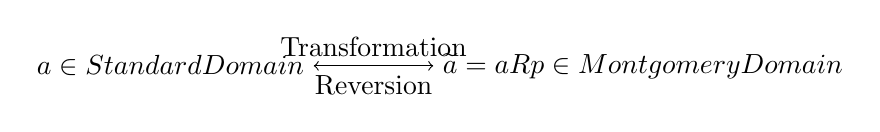
\begin{tikzpicture}
		\node (A) at (0,0) {$a \in \text{Standard Domain}$};
		\node (B) at (6,0) {$\widetilde{a} = aR \mod p \in \text{Montgomery Domain}$};
		\draw[->] (A) -- (B) node[midway,above] {Transformation};
		\draw[->] (B) -- (A) node[midway,below] {Reversion};
	\end{tikzpicture}
\end{center}

\subsection{Montgomery Reduction}
Montgomery Reduction transforms the problem of modular multiplication into a more efficiently computable form by redefining the multiplication operation in terms of alternative representations of the numbers involved. Specifically, it introduces a mapping function based on a chosen constant $R$, which is co-prime to the modulus $m$ and typically a power of $2$ for computational efficiency.
\vspace{8pt}
\begin{example}
Compute \[
3\cdot 7\bmod{11}
\] \begin{proof}[\sol]
Let $R=2^4=16>11$. 

\begin{itemize}
\item[] \textbf{Step 1: Transformation to Montgomery Space}

We transform $X=3$ and $Y=7$ into Montgomery space: \begin{align*}
X'&=3\cdot R\bmod 11=3\cdot16\bmod 11 = 4 \\
Y'&=7\cdot R\bmod 11=7\cdot16\bmod 11 = 2
\end{align*} Here, $X'$ and $Y'$ are the Montgomery representations of $X$ and $Y$, respectively.
\item[] \textbf{Step 2: Montgomery Multiplication}

Note that $R^{-1}$ satisfies $RR^{-1}\equiv 1\pmod{11}$: \begin{align*}
	R^{-1}R=R^{-1}\cdot 2^4&\equiv 1\pmod{11} \\
	R^{-1}R=R^{-1}\cdot 5&\equiv 1\pmod{11}\quad\because 16\equiv 5\pmod{11} \\
	R^{-1}&\equiv 9\pmod{11}\quad\because 5\cdot 9\equiv 1\pmod{11} \\
\end{align*} 
We multiply $X'$ and $Y'$ but the result is in Montgomery form: for $Z'=X'Y'$, \[
Z'R^{-1}\bmod 11 = 8\cdot 9\bmod 11 = 6.
\]
\item[] \textbf{Step 3: Conversion Back from Montgomery Space}
\end{itemize}
\end{proof}
\end{example}
\vspace{8pt}
\begin{tcolorbox}[colframe=defcolor,title={\color{white}\bf The Montgomery Representation and the inverse Montgomery Transformation}]
\begin{definition}
The Montgomery representation of a finite field element $x\in\intco{0,N}$, \[
\fullfunction{M}{\Z_N}{\Z_N}{x}{(xR)\bmod N},
\] is a mapping from the standard representation to the Montgomery domain, where $R=2^k$ for some $k$, a constant such that $R\geq m$ $\gcd(R,m)=1$.

The inverse Montgomery transformation, \[
\fullfunction{M^{-1}}{\Z_N}{\Z_N}{u}{(uR^{-1})\bmod N},
\] is a mapping back form the Montgomery domain to the standard representation, where $R^{-1}$ is the modular inverse of $R$ modulo $m$, \ie, $RR^{-1}\equiv 1\pmod{m}$.
\end{definition}
\end{tcolorbox}

\newpage
\begin{tcolorbox}[colframe=defcolor,title={\color{white}\bf The Montgomery Reduction}]
\begin{definition}
Define a mapping \textbf{Montgomery Reduction} $\mathsf{MontRed}:\Z_{NR}\to\Z_{N}$ as follows: \[
\mathsf{MontRed}(x):=xR^{-1}\bmod N,
\] for $x\in\intco{0,NR}$, where \begin{enumerate}[(i)]
\item $R=2^{wt}>N$
\item $\gcd(R=2^{wt}, N)=1$.
\end{enumerate}
\end{definition}	
\end{tcolorbox}
\begin{itemize}
	\item Let \( \mathcal{M} : \mathbb{F}_p \to \widetilde{\mathbb{F}}_p \) be the Montgomery transformation function, where \( \mathcal{M}(a) = aR \mod p \) transforms an element from the standard domain \( \mathbb{F}_p \) to the Montgomery domain \( \widetilde{\mathbb{F}}_p \).
	\item Let \( \mathcal{M}^{-1} : \widetilde{\mathbb{F}}_p \to \mathbb{F}_p \) be the inverse Montgomery transformation function, where \( \mathcal{M}^{-1}(\widetilde{a}) = \widetilde{a}R^{-1} \mod p \) transforms an element back from the Montgomery domain \( \widetilde{\mathbb{F}}_p \) to the standard domain \( \mathbb{F}_p \).
\end{itemize}

\newpage
\section{Montgomery Reduction}

\begin{tcolorbox}[colframe=defcolor,title={\color{white}\bf Montgomery From}]
\begin{definition}
Consider a element of finite field $\F_N$: \[
x\in\intco{0,N}.
\] Montgomery representation is defined as: \[
[x]:=(xR)\bmod N,
\] where \begin{enumerate}[(i)]
\item $R=2^{wt}>N$
\item $\gcd(R=2^{wt}, N)=1$.
\end{enumerate}
\end{definition}	
\end{tcolorbox}

\begin{tcolorbox}[colframe=defcolor,title={\color{white}\bf Montgomery Reduction}]
\begin{definition}
Define a mapping \textbf{Montgomery Reduction} $\mathsf{MontRed}:\Z_{NR}\to\Z_{N}$ as follows: \[
\mathsf{MontRed}(u):=uR^{-1}\bmod N,
\] for $u\in\set{[u]: u\in \F_N}$.
\end{definition}	
\end{tcolorbox}
\begin{remark}
\ \begin{itemize}
\item $\MontRed (xR^2\bmod N)=[x]$
\item $\MontRed ([x])=x$
\end{itemize}
\end{remark}

\begin{algorithm}[H]
\DontPrintSemicolon
\caption{Montgomery Reduction: $\MontRed(x)=xR^{-1}\bmod N$}
\BlankLine
\Comment{$R^{-1}$ satisfies $RR^{-1}\equiv 1\pmod N$}
\Comment{$N^{-1}$ satisfies $NN^{-1}\equiv 1\pmod R$}
\KwIn{$(xR)\bmod N$ with the pre-computed values $R$, $N^{-1}$}
\KwOut{$\MontRed(x)=xR^{-1}\bmod N$}
\BlankLine
$s\gets(x\bmod R)\cdot N^{-1}\bmod R$\tcp*{$s\gets (x\land \one^{wt})\cdots N^{-1}\bmod R$}
$t\gets(x+s\cdot N) / R$\tcp*{$t\gets (x+sN)\gg wt$}
\If{$t\geq N$}{
	$t\gets t-N$
} \Return $t$\;
\end{algorithm}
\begin{proof}[Correctness for Montogmery Reduction]
\begin{align*}
s&=(x\bmod R)\cdot N^{-1}\bmod R, \\
sN&\equiv (x\bmod R)N^{-1}N\pmod R \\
&\equiv xN^{-1}N\pmod R \\
\end{align*}
\end{proof}

